本节介绍将北京的空气质量数据进行离散化, 按照空气质量分级表存, 计算出每个级别对应
的挺熟, 并将结果以饼图的形式进行可视化. 对每一个PM来源均分别进行饼图可视化, 以便于比较.

\subsection{空气质量分级标准}
参考如表~\ref{tab:空气质量分级标准}空气质量分级标准:
\begin{table}[ht!]
    \centering
    \begin{tabular}{|l|l|}
        \hline
        空气质量指数(AQI) & 空气质量指数级别(状况)              \\
        \hline
        \hline
        0-50        & Excellent(优)              \\
        51-100      & Good(良)                   \\
        101-150     & Lightly Polluted(轻度污染)    \\
        151-200     & Moderately Polluted(中度污染) \\
        201-300     & Heavily Polluted(重度污染)    \\
        300+        & Severely Polluted(严重污染)   \\
        \hline
    \end{tabular}
    \caption{空气质量分级标准}
    \label{tab:空气质量分级标准}
\end{table}

\subsection{实现介绍}
由于不同观测数据来源的PM数据有差异, 故使用如下函数对各站点PM数据分别进行离散化.
\begin{lstlisting}[language=Python]
    # Discretize PM_Dongsi into PM_Dongsi_AQI:
    def discretize_pm(column, discretized_column):
        for row in column:
            if 0 <= row <= 50:
                discretized_column.append(aqis.excellent._value_)
            elif 51 <= row <= 100:
                discretized_column.append(aqis.good._value_)
            elif 101 <= row <= 150:
                discretized_column.append(aqis.lightly_polluted._value_)
            elif 151 <= row <= 200:
                discretized_column.append(aqis.moderately_polluted._value_)
            elif 201 <= row <= 300:
                discretized_column.append(aqis.heavily_polluted._value_)
            elif row > 300:
                discretized_column.append(aqis.severely_polluted._value_)
            else:
                # Handle NaN value.
                discretized_column.append(row)
\end{lstlisting}

数据可视化部分, 首先统计了各空气质量等级的天数:
\begin{lstlisting}[language=Python]
    classes = [self.aqicategories.excellent._value_,
    self.aqicategories.good._value_,
    self.aqicategories.lightly_polluted._value_,
    self.aqicategories.moderately_polluted._value_,
    self.aqicategories.heavily_polluted._value_,
    self.aqicategories.severely_polluted._value_]

    def count(col):
    '''
    Count AQI categories. Ignore NaN values.
    '''
    rslt = [0 for i in range(len(classes))]
    for row in col:
     if row in classes:
         rslt[classes.index(row)] += 1
    return rslt
\end{lstlisting}

然后对数据绘制饼图进行可视化:
\begin{lstlisting}[language=Python]
    data_dongsi = count(df["PM_Dongsi_AQI"])
    data_dongsihuan = count(df["PM_Dongsihuan_AQI"])
    data_nongzhanguan = count(df["PM_Nongzhanguan_AQI"])
    data_us = count(df["PM_US Post_AQI"])

    def draw_sub_pie(data, ax_x, ax_y):
    '''
    Draw subplot of pie.
    '''
    def get_absolute(pct, allvals):
        '''
        Get absolute value of days from percentage.
        '''
        absolute = int(np.round(pct/100.*np.sum(allvals)))
        return "{:.1f}%\n({:d} days)".format(pct, absolute)

    wedges, texts, autotexts = ax.pie(data, wedgeprops=dict(
        width=0.618), startangle=90, autopct=lambda pct: get_absolute(pct, data))
    bbox_props = dict(boxstyle="square,pad=0.3",
                      fc="w", ec="k", lw=0.72)
    kw = dict(arrowprops=dict(arrowstyle="-"),
              bbox=bbox_props, zorder=0, va="center")

    # Compute angle of label line
    for i, p in enumerate(wedges):
        ang = (p.theta2 - p.theta1)/2. + p.theta1
        y = np.sin(np.deg2rad(ang))
        x = np.cos(np.deg2rad(ang))
        horizontalalignment = {-1: "right", 1: "left"}[int(np.sign(x))]
        connectionstyle = "angle,angleA=0,angleB={}".format(ang)
        kw["arrowprops"].update({"connectionstyle": connectionstyle})
        ax.annotate(classes[i] + " " + zh_classes[i], xy=(x, y), xytext=(
            1.35*np.sign(x), 1.2*y), horizontalalignment=horizontalalignment, **kw)

    
    # Draw PM_Dongsi pie plot.
    fig, ax = plt.subplots(figsize=(
        12, 8), subplot_kw=dict(aspect="equal"))
    draw_sub_pie(data_dongsi, 0, 0)
    ax.set_title("Dongsi PM AQI")
    plt.show()
    
    ...
\end{lstlisting}

\subsection{处理结果}
在样例数据上进行处理得到的结果如下, 由于新增四列后表格太宽, 所以进行了换行:
\begin{lstlisting}
    ...  PM_Dongsi  PM_Dongsihuan  PM_Nongzhanguan  PM_US Post  ...    
    ...                                                         ...
    ...        NaN            NaN              NaN         NaN  ...    
    ...        NaN            NaN              NaN         NaN  ...    
    ...        NaN            NaN              NaN         NaN  ...    
    ...        NaN            NaN            500.0         NaN  ...    
    ...        NaN           39.0              NaN         NaN  ...    
    ...        NaN            NaN              NaN      1818.0  ...    
    ...        NaN          500.0              NaN       383.0  ...    
    ...       17.0            NaN              NaN        12.0  ...    
    ...        NaN            NaN              NaN         NaN  ...    
    ...        NaN            NaN              NaN         NaN  ...    

     PM_Dongsi_AQI  PM_Dongsihuan_AQI PM_Nongzhanguan_AQI     PM_US Post_AQI
                                                                            
               NaN                NaN                 NaN                NaN
               NaN                NaN                 NaN                NaN
               NaN                NaN                 NaN                NaN
               NaN                NaN   Severely Polluted                NaN
               NaN          Excellent                 NaN                NaN
               NaN                NaN                 NaN  Severely Polluted
               NaN  Severely Polluted                 NaN  Severely Polluted
         Excellent                NaN                 NaN          Excellent
               NaN                NaN                 NaN                NaN
               NaN                NaN                 NaN                NaN
\end{lstlisting}
可以看到对非NaN的值, 都进行了正确的对应离散化.

在完整的Bejing PM数据集上处理的各观测数据的统计信息如下:
\begin{lstlisting}
PM_Dongsi statistics:
    Excellent[10576]
    Good[6268]
    Lightly Polluted[3578]
    Moderately Polluted[1942]
    Heavily Polluted[1910]
    Severely Polluted[778]

PM_Dongsihuan statistics:
    Excellent[8104]
    Good[5408]
    Lightly Polluted[3143]
    Moderately Polluted[1683]
    Heavily Polluted[1416]
    Severely Polluted[754]

PM_Nongzhanguan statistics:
    Excellent[10730]
    Good[6259]
    Lightly Polluted[3408]
    Moderately Polluted[1934]
    Heavily Polluted[1697]
    Severely Polluted[903]

PM_US Post statistics:
    Excellent[20050]
    Good[12576]
    Lightly Polluted[7414]
    Moderately Polluted[4274]
    Heavily Polluted[4016]
    Severely Polluted[2057]
\end{lstlisting}

\subsection{可视化结果}
PM\_Dongsi的可视化结果如图~\ref{fig:PMDongsi的AQI离散化}.

\begin{figure}[ht!]
    \centering
    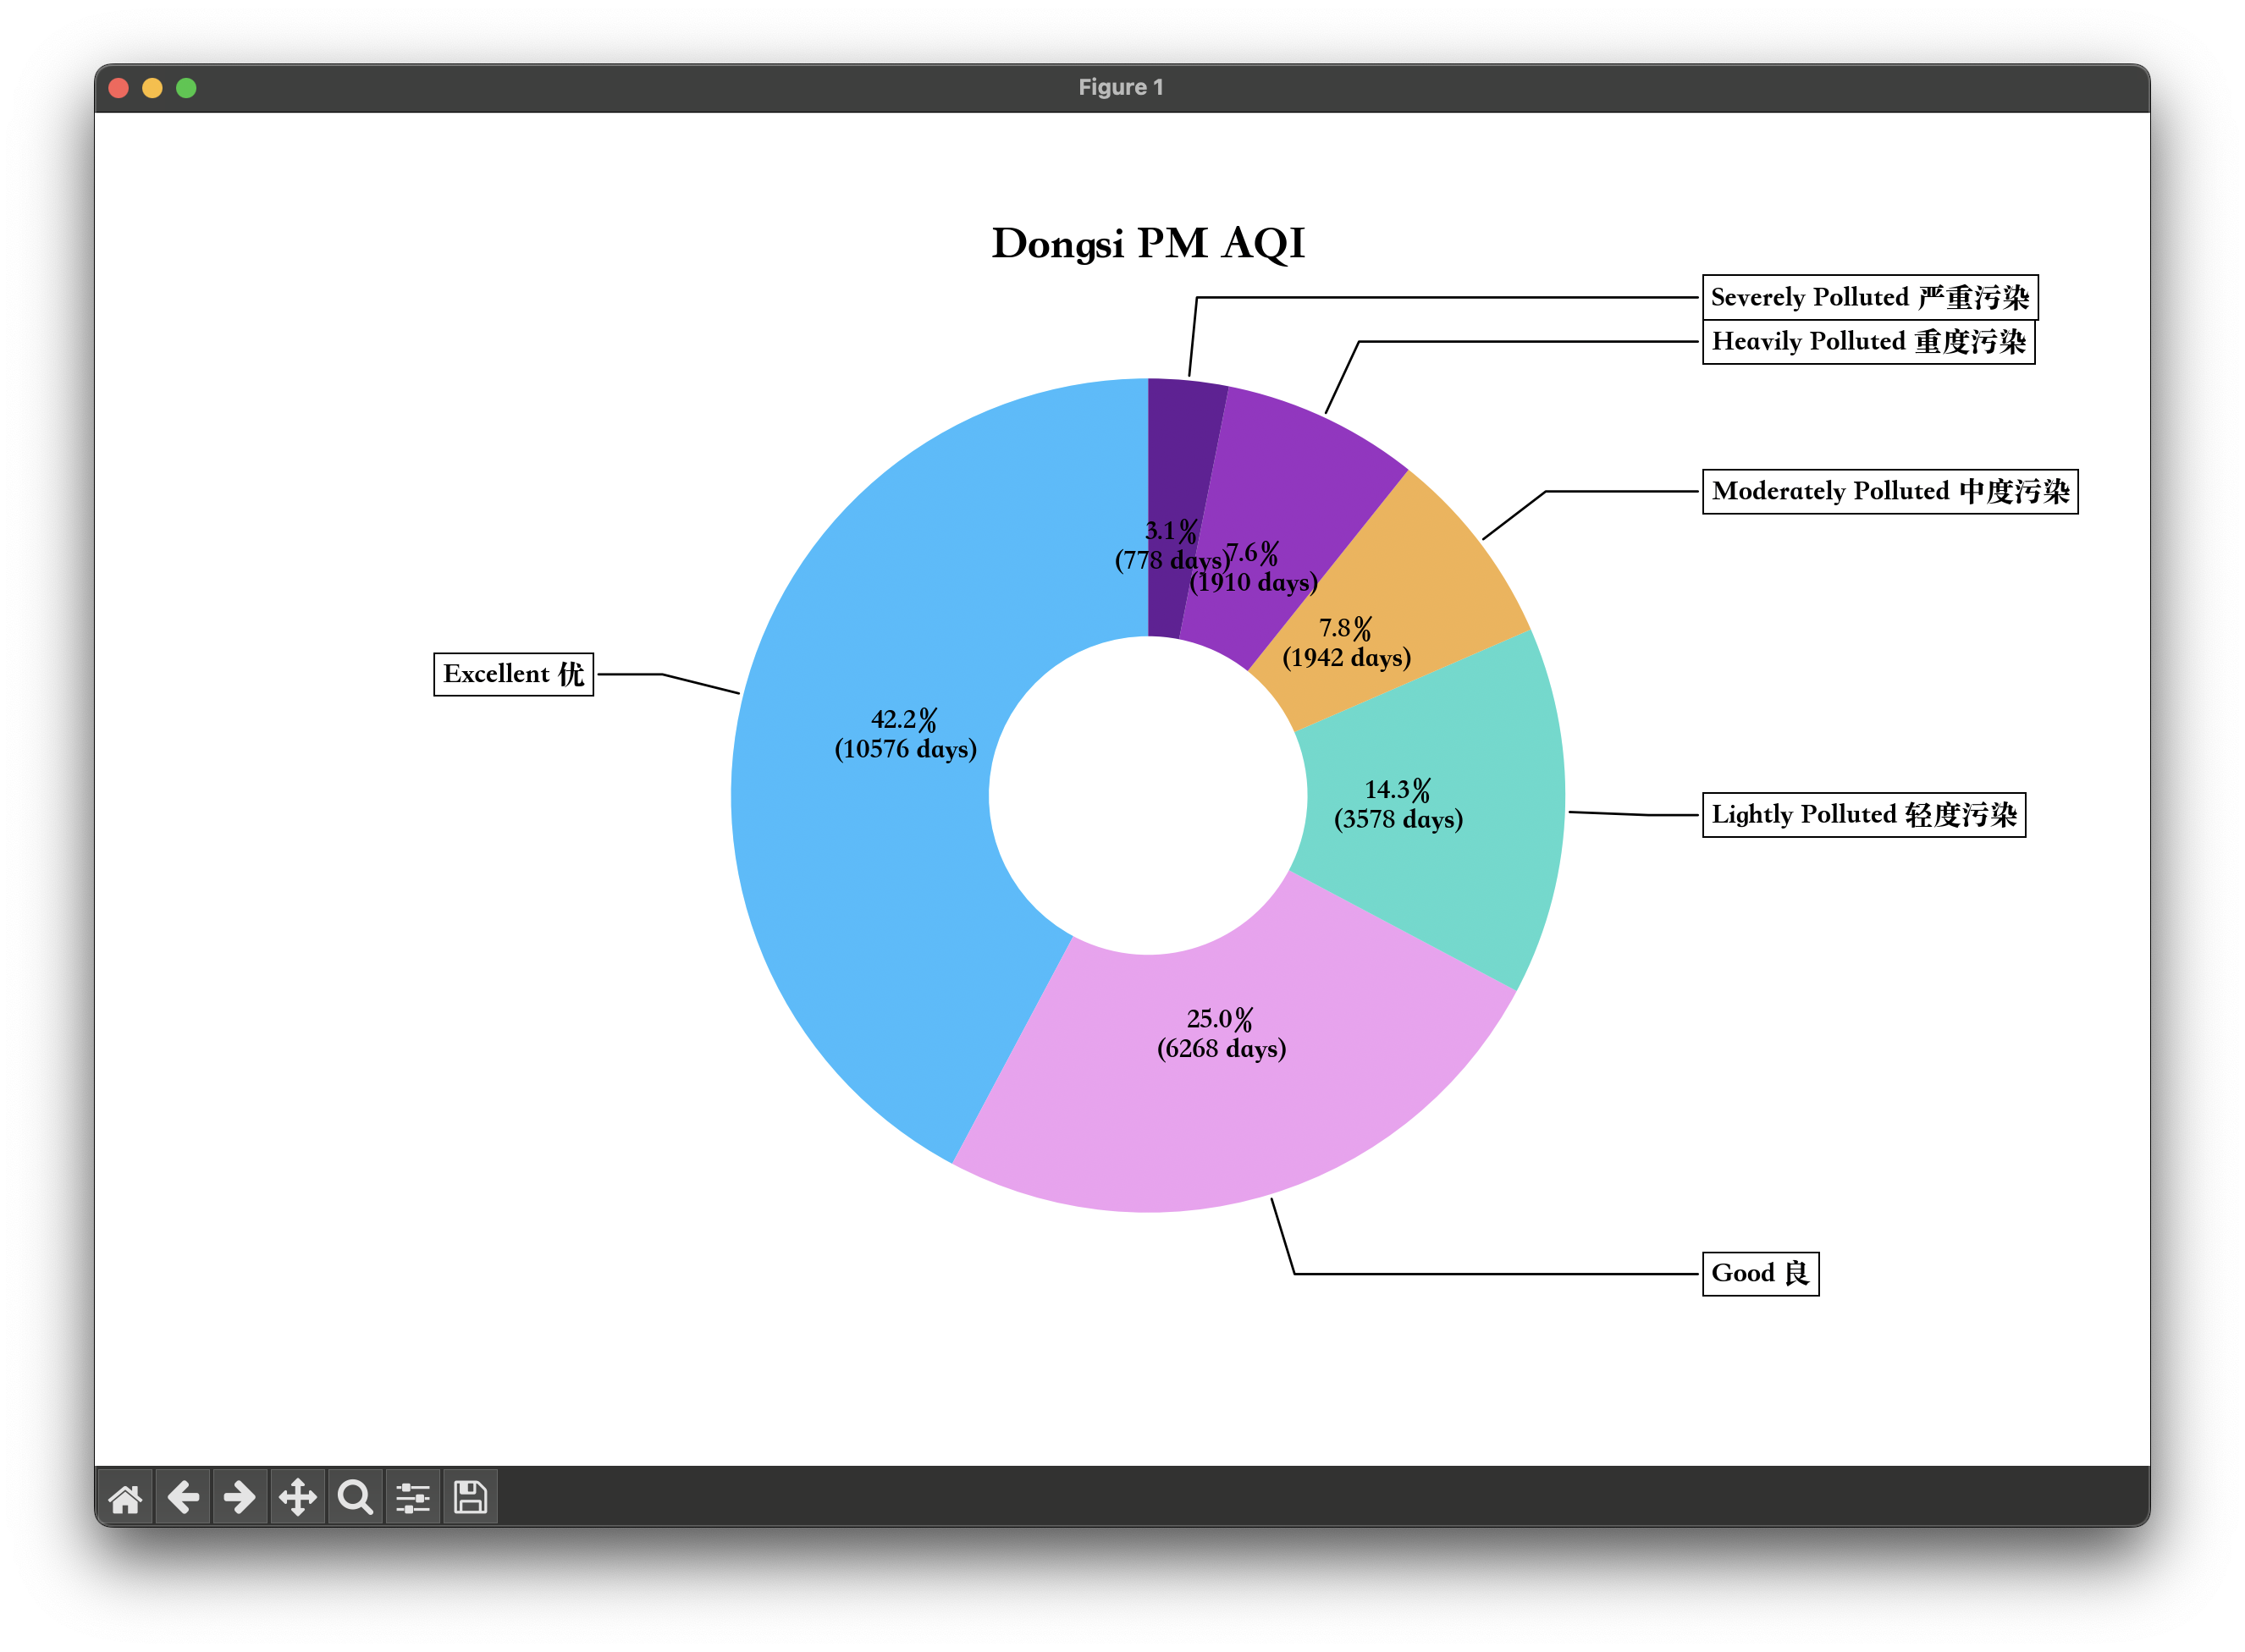
\includegraphics[width=0.8\textwidth]{discretize-aqi-dongsi.png}
    \caption{PM\_Dongsi的AQI离散化}
    \label{fig:PMDongsi的AQI离散化}
\end{figure}

PM\_Dongsihuan的可视化结果如图~\ref{fig:PMDongsihuan的AQI离散化}

\begin{figure}[ht!]
    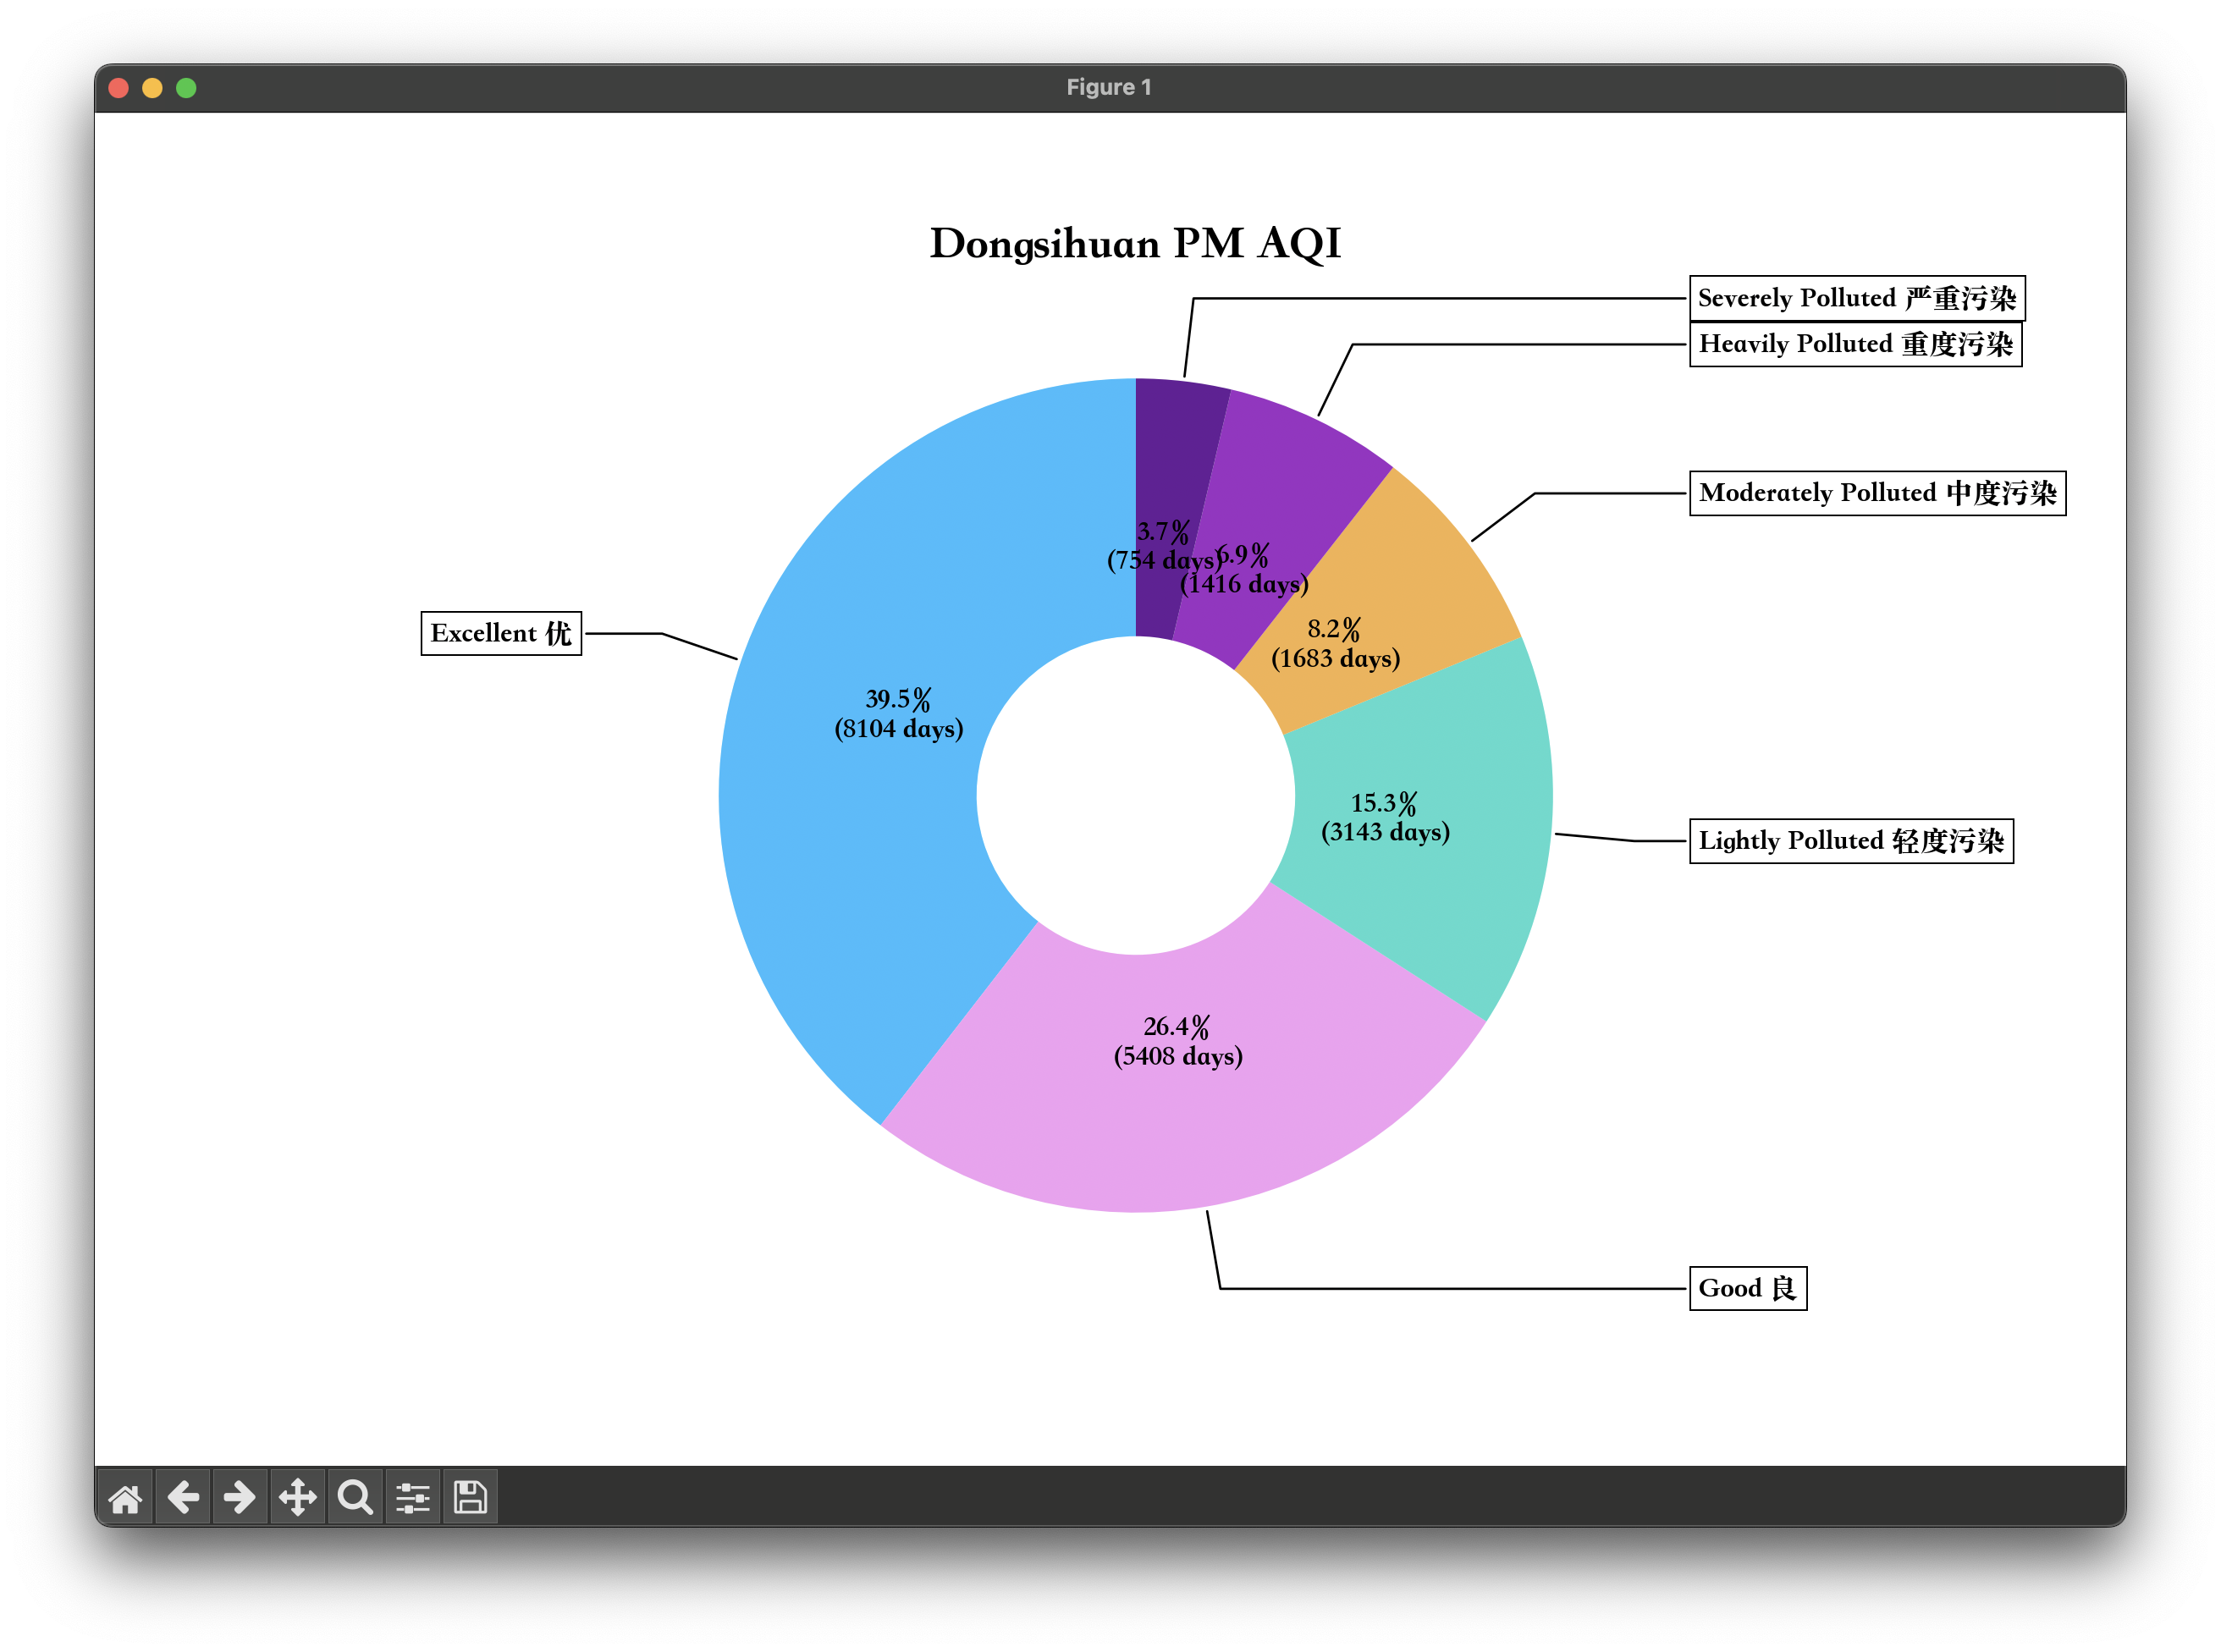
\includegraphics[width=0.8\textwidth]{discretize-aqi-dongsihuan.png}
    \centering
    \caption{PM\_Dongsihuan的AQI离散化}
    \label{fig:PMDongsihuan的AQI离散化}
\end{figure}

PM\_Nongzhanguan的可视化结果如图~\ref{fig:PMNongzhanguan的AQI离散化}
\begin{figure}[ht!]
    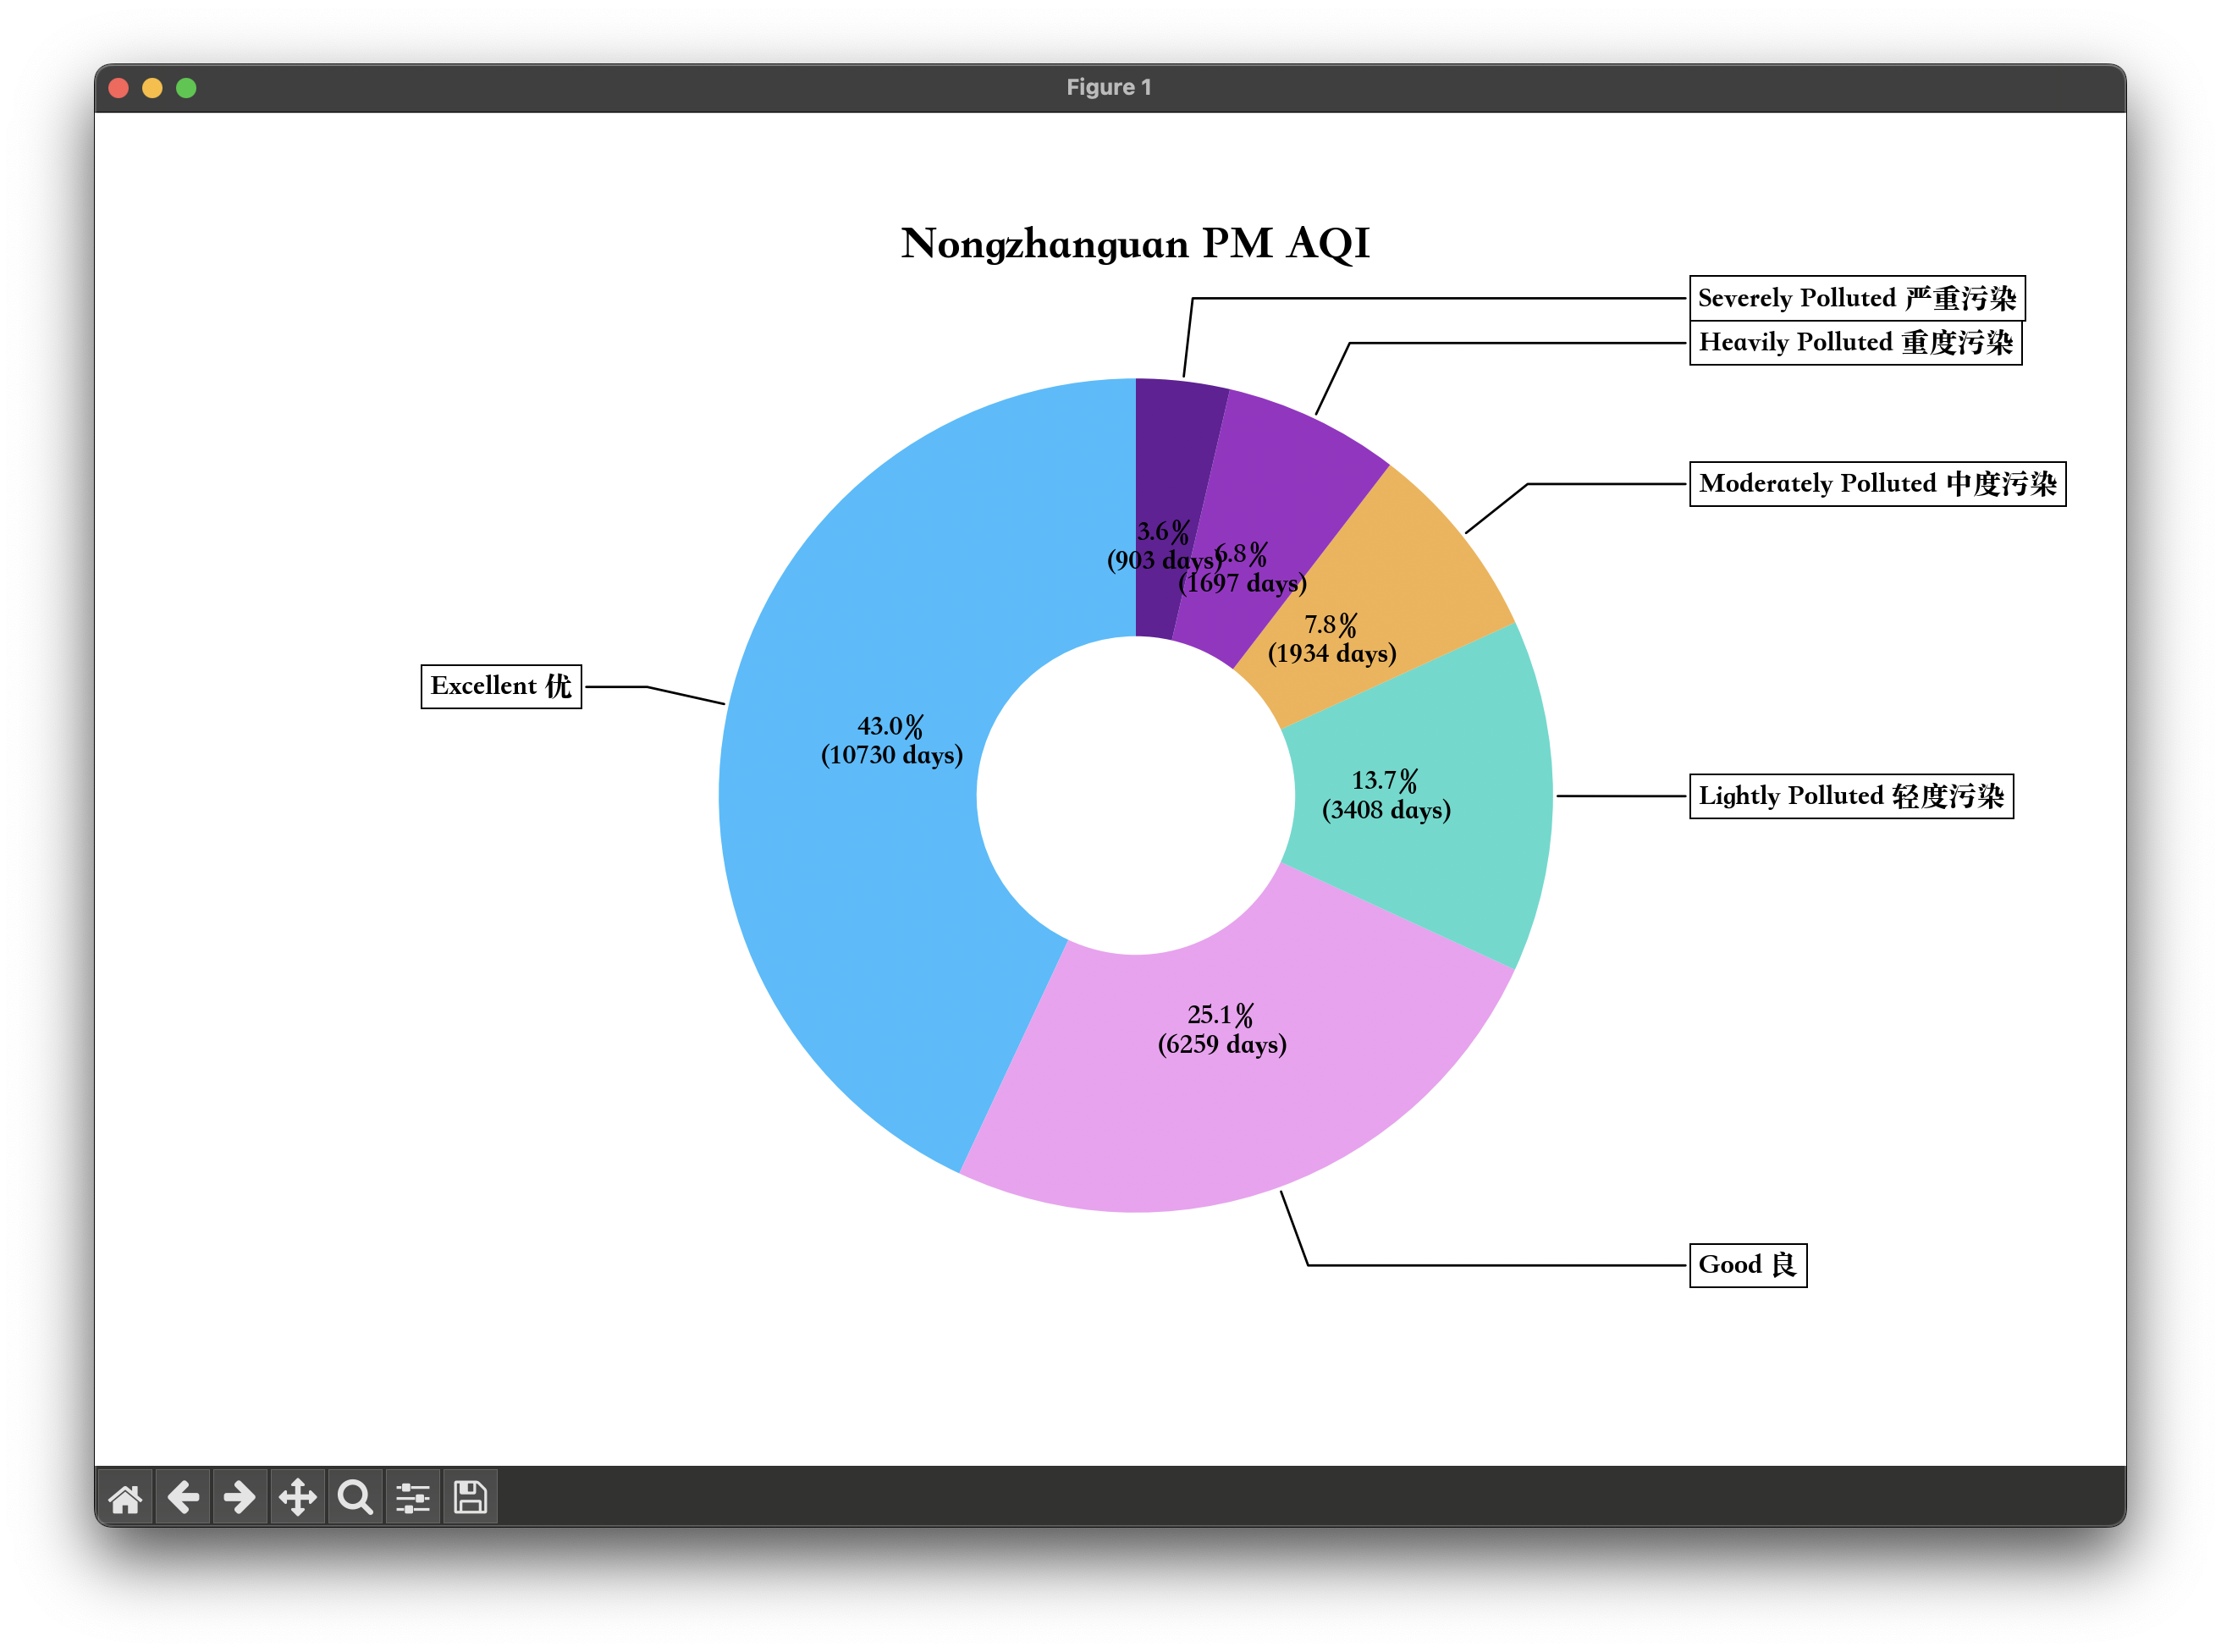
\includegraphics[width=0.8\textwidth]{discretize-aqi-nongzhanguan.png}
    \centering
    \caption{PM\_Nongzhanguan的AQI离散化}
    \label{fig:PMNongzhanguan的AQI离散化}
\end{figure}

PM\_US Post的可视化结果如图~\ref{fig:PMUS Post的AQI离散化}
\begin{figure}[ht!]
    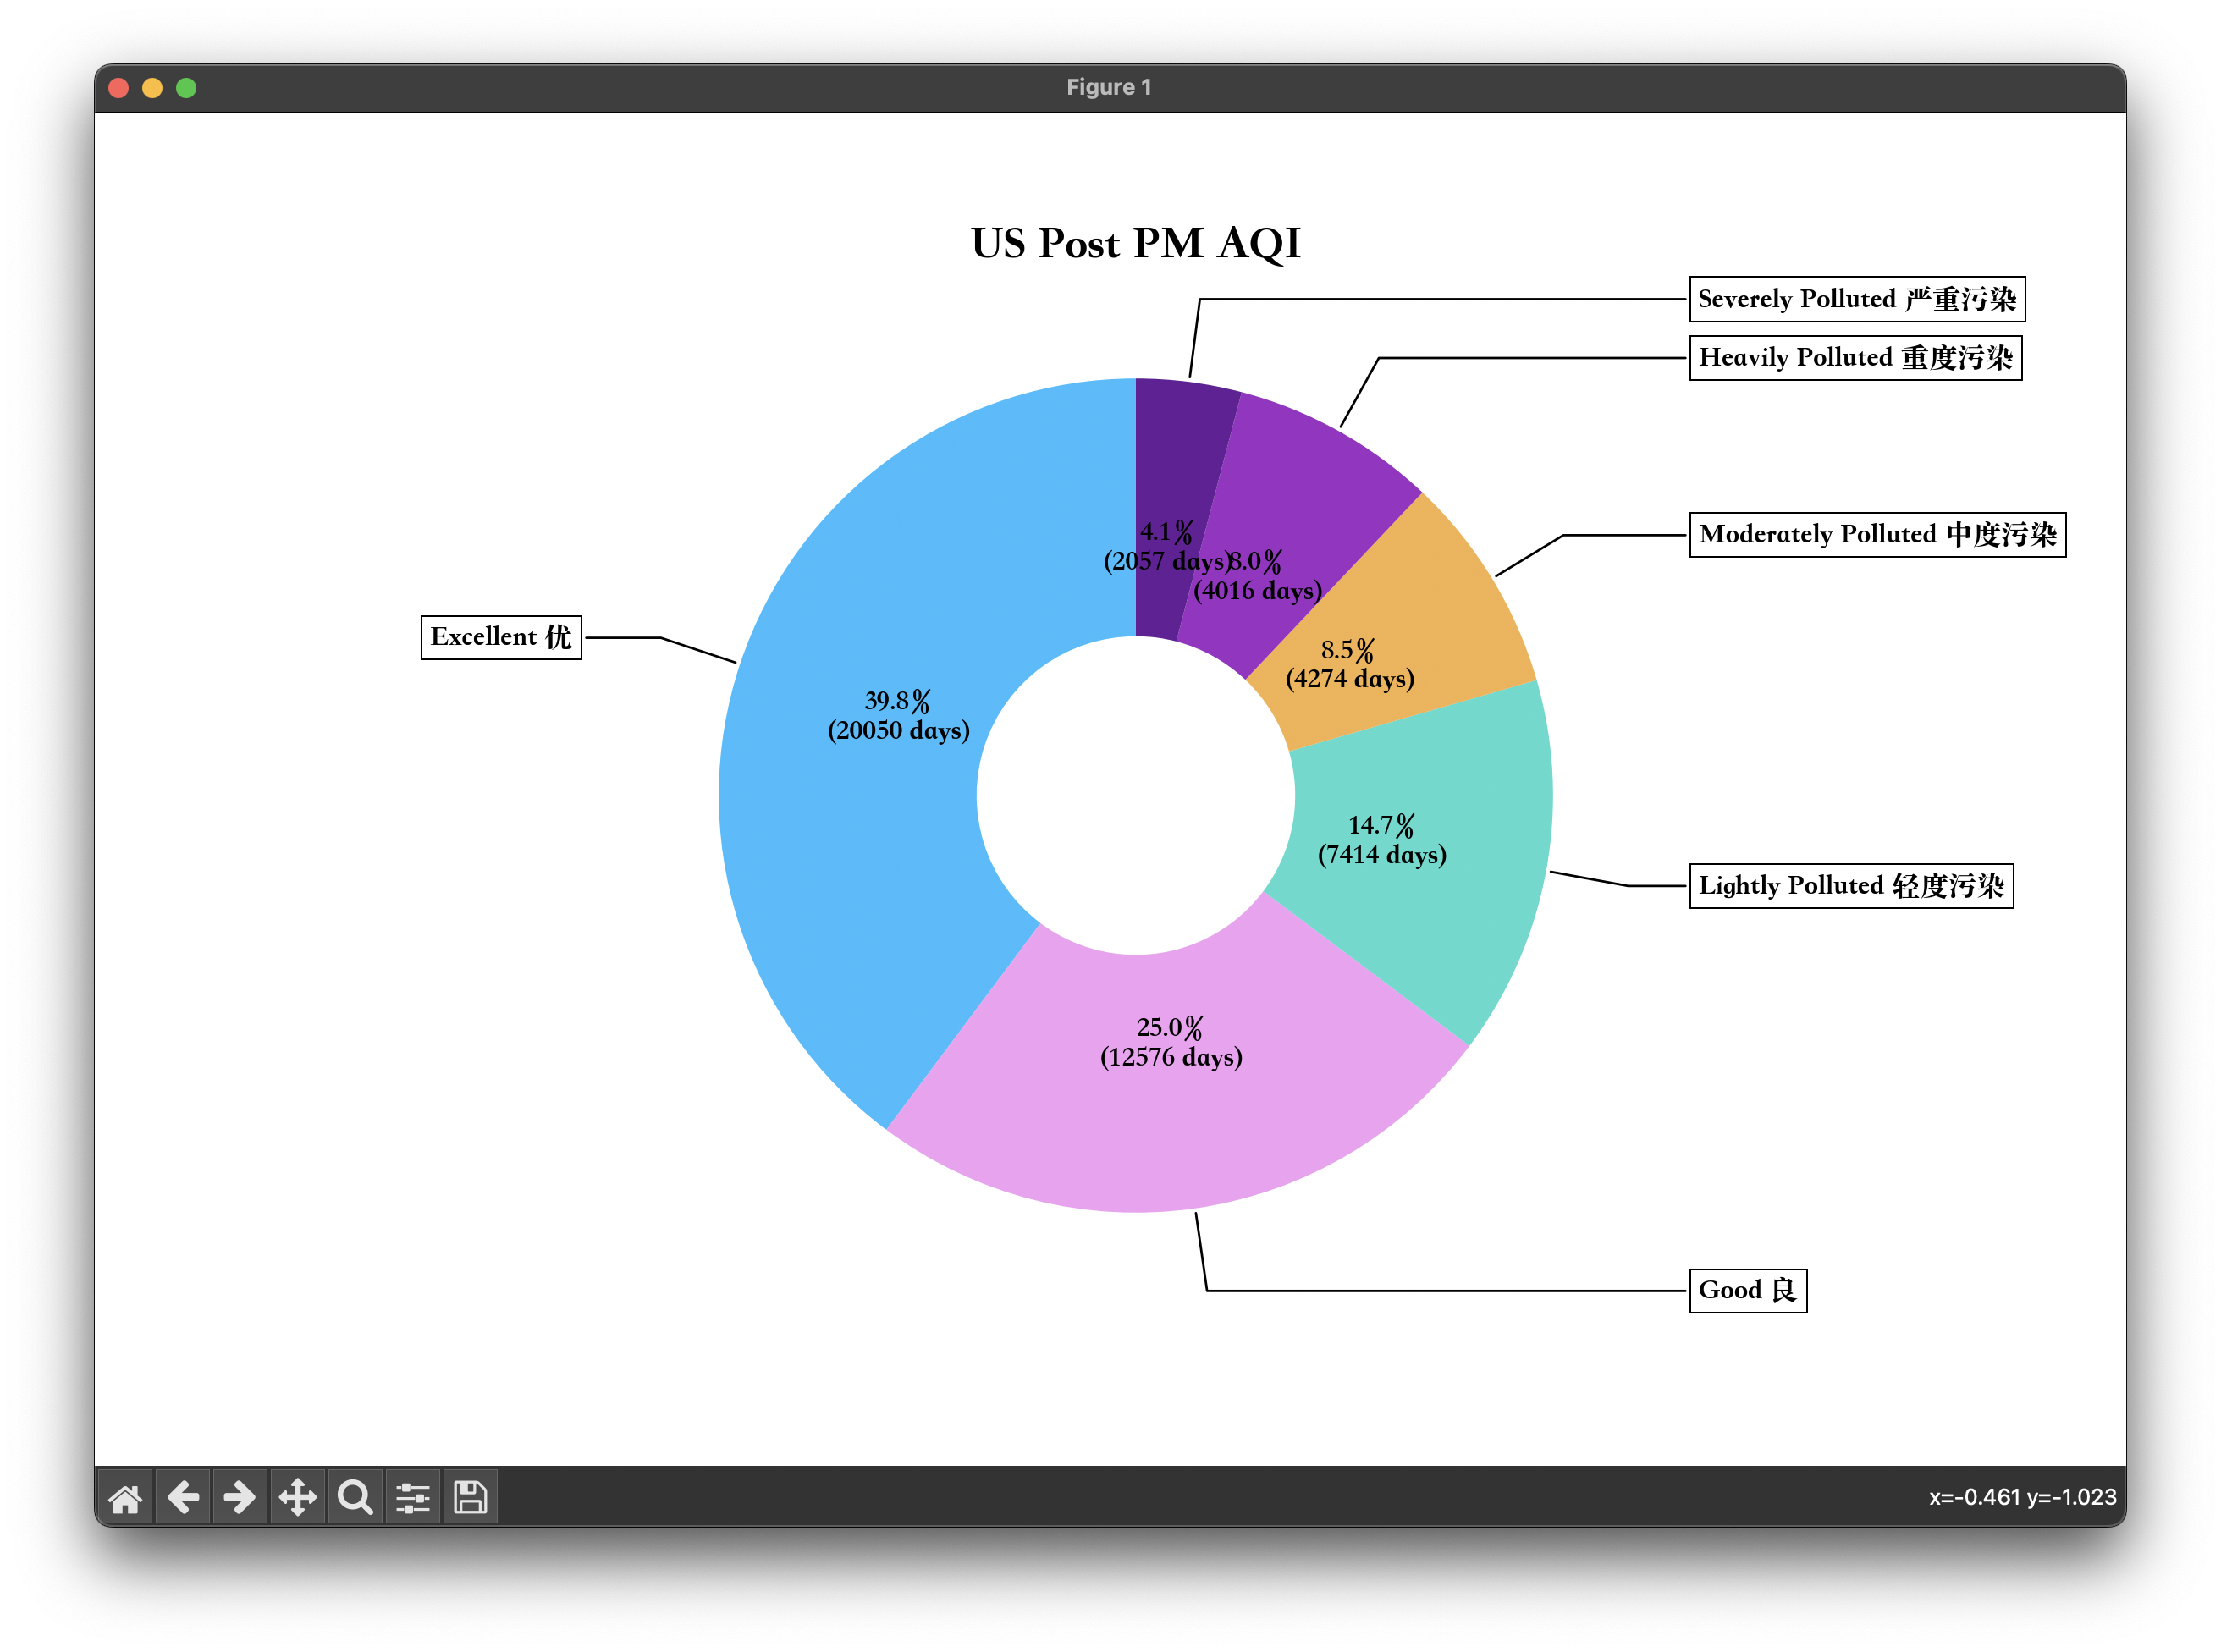
\includegraphics[width=0.8\textwidth]{discretize-aqi-us-post.png}
    \centering
    \caption{PM\_US Post的AQI离散化}
    \label{fig:PMUS Post的AQI离散化}
\end{figure}
